
\frame { \frametitle{ LSST:uniform sky survey }
\begin{columns}
\column{0.5\textwidth}
\vspace {-5cm}
 \\
An optical/near-IR survey of half the sky in ugrizy bands to r~27.5 (36 nJy) based on 825 visits over  a 10-year period: {\em deep wide fast}.
%It’s about 5,000 sq. deg. per night, *twice*, on
%average. That is, about 1,000 visits per night on average. You return to
%the same position on the sky in about 3-4 nights (in any band). Btw, it’s
%a nice coincidence worth remembering that the total exposure time per
%position over 10 years (in all bands) is equal to about one observing night.
\begin{itemize}
\item 90\% of time  spent on  uniform survey: every 3-4 nights, the whole observable sky scanned twice per night
\item	~100 PB of data: about a billion 16 Mpix images, enabling measurements\\ {\color{cyan} for 40 billion objects! }
\end{itemize}
{\tiny see also \url{http://www.lsst.org} and \cite{2008arXiv0805.2366I}-arXiv:0805.2366}

\column{0.5\textwidth}
	 \includegraphics[width=1.1\textwidth]{images/coverage}\\
{\bf 10-year simulation : number of visits in u,g,r band (Aitoff projection of eq. coordinates) }\\
\end{columns}

}



\frame{\frametitle{Science Platform Vision to Reality }
\vspace{-5pt}
Vision: \citeds{LSE-319} --- Design: \citeds{LDM-542} --- Test: \citeds{DMTR-51} at NCSA

\begin{columns}
\begin{column}{0.7\textwidth}
\includegraphics[width=1\textwidth]{images/psfnb}
\end{column}
\begin{column}{0.3\textwidth}
\vspace{-7cm}
\\
Portal/Browser\\
Notebooks\\
Web API\\
(Batch)\\
\hspace{-1.5cm} \includegraphics[width=1.3\textwidth]{images/firefly}\\
\hspace{0.1cm} {\tiny \bf Images Krughoff($\leftarrow$) and Wu ($\uparrow$)}
\end{column}
\end{columns}

}


\frame {\frametitle{ Data management }
\begin{columns}
\column{0.7\textwidth}
      \includegraphics[width=1.0\textwidth]{images/dm2018}\\
\column{0.3\textwidth}
 \\
\vspace{-5cm}

 DM Mission :\\
    {\em  Stand up operable, maintainable, quality services to deliver high-quality LSST data products for science, all on time and within reasonable cost.}\\
\end{columns}
    \vspace{7pt}
LSST DM development is distributed across the Americas.\\

{\color{blue} Plus we have partners like IN2P3}\\
See Management Plan \citeds{LDM-294}.

}



\frame {\frametitle{Build and Deploy with a view to Ops}
\vspace{-1cm}
\begin{columns}
\column{0.5\textwidth}
\begin{center}
\vspace{-0.5cm}
      \includegraphics[width=1.0\textwidth]{images/DMSDeployment}\\
\vspace{-5.3cm}
      \includegraphics[width=0.8\textwidth]{images/linesOfCode}\\
\end{center}
\column{0.5\textwidth}
 \\
\vspace{0.2cm}
DM must build everything to get LSST data products---as described in \citeds{LSE-163}---to end users.
\begin{itemize}
\item Large data sets (20\,TB/night)
\item Complex analysis with small systematics
\item Science alerts issued within one minute
\end{itemize}
$\sim{}^3\!/_4$ million lines of code/comments (C++/Python/Java/JavaScript/Kotlin)\\
See SPIE paper by \cite{2018SPIE10707E..09J}\\
\vspace{2pt}
Architecture and Components  \citeds{LDM-148}.\\
 Concept of Operations \citeds{LDM-230}.\\
\vspace{1pt}
{\tiny Upper diagram courtesy K-T Lim, \citeds{LDM-148}. }\\
{\tiny Lower diagram by Tim Jenness; covers only the Science Pipelines
codebase.}
\end{columns}
}

\frame {\frametitle{All comes down to image- SDSS example }
	\vspace{-1mm}
	\begin{columns}
		\column{0.5\textwidth}
		\vspace{-2mm}
	      \includegraphics[width=1.0\textwidth]{images/SDSScosmos}\\
		      \column{0.5\textwidth}
		      \\
		       \vspace{1cm}
	       Nice colors \cite{2004PASP..116..133L}\\
	       $\approx  3.5 \arcmin$\\
		       \vspace{20mm}
	       {\tiny \bf{Image  Robert Lupton}}
	       \end{columns}
}
\frame {\frametitle{Hyper Suprime Cam (HSC) on Subaru }
	\vspace{-1mm}
	\begin{columns}
		\column{0.5\textwidth}
		\vspace{-2mm}
	      \includegraphics[width=1.0\textwidth]{images/HSCcosmos}\\
		      \column{0.5\textwidth}
		       \\
		       HSC image (COSMOS) from g,r(1.5 hrs) ,i(3 hrs) PSF matched co-add ($\approx 27.5$)\\
		       \vspace{3mm}
		       Processed with  {\em LSST Stack} \url{https://pipelines.lsst.io/}\\
		       \vspace{3mm}
YES the Pipelines are already in use with other facilities like Hyper Suprime-Cam.\\
\vspace{3mm}
Still working on performance, algorithmic enhancements, orchestration, etc.\\
\vspace{3mm}
Design \citeds{LDM-151}; Test Specs \citeds{LDM-533, LDM-534}; Test Reports \citeds{DMTR-52, DMTR-53}\\
	       {\tiny \bf{Image HSC collaboration,  Robert Lupton}}
	       \end{columns}
       }



\frame{\frametitle{LSST Data products }
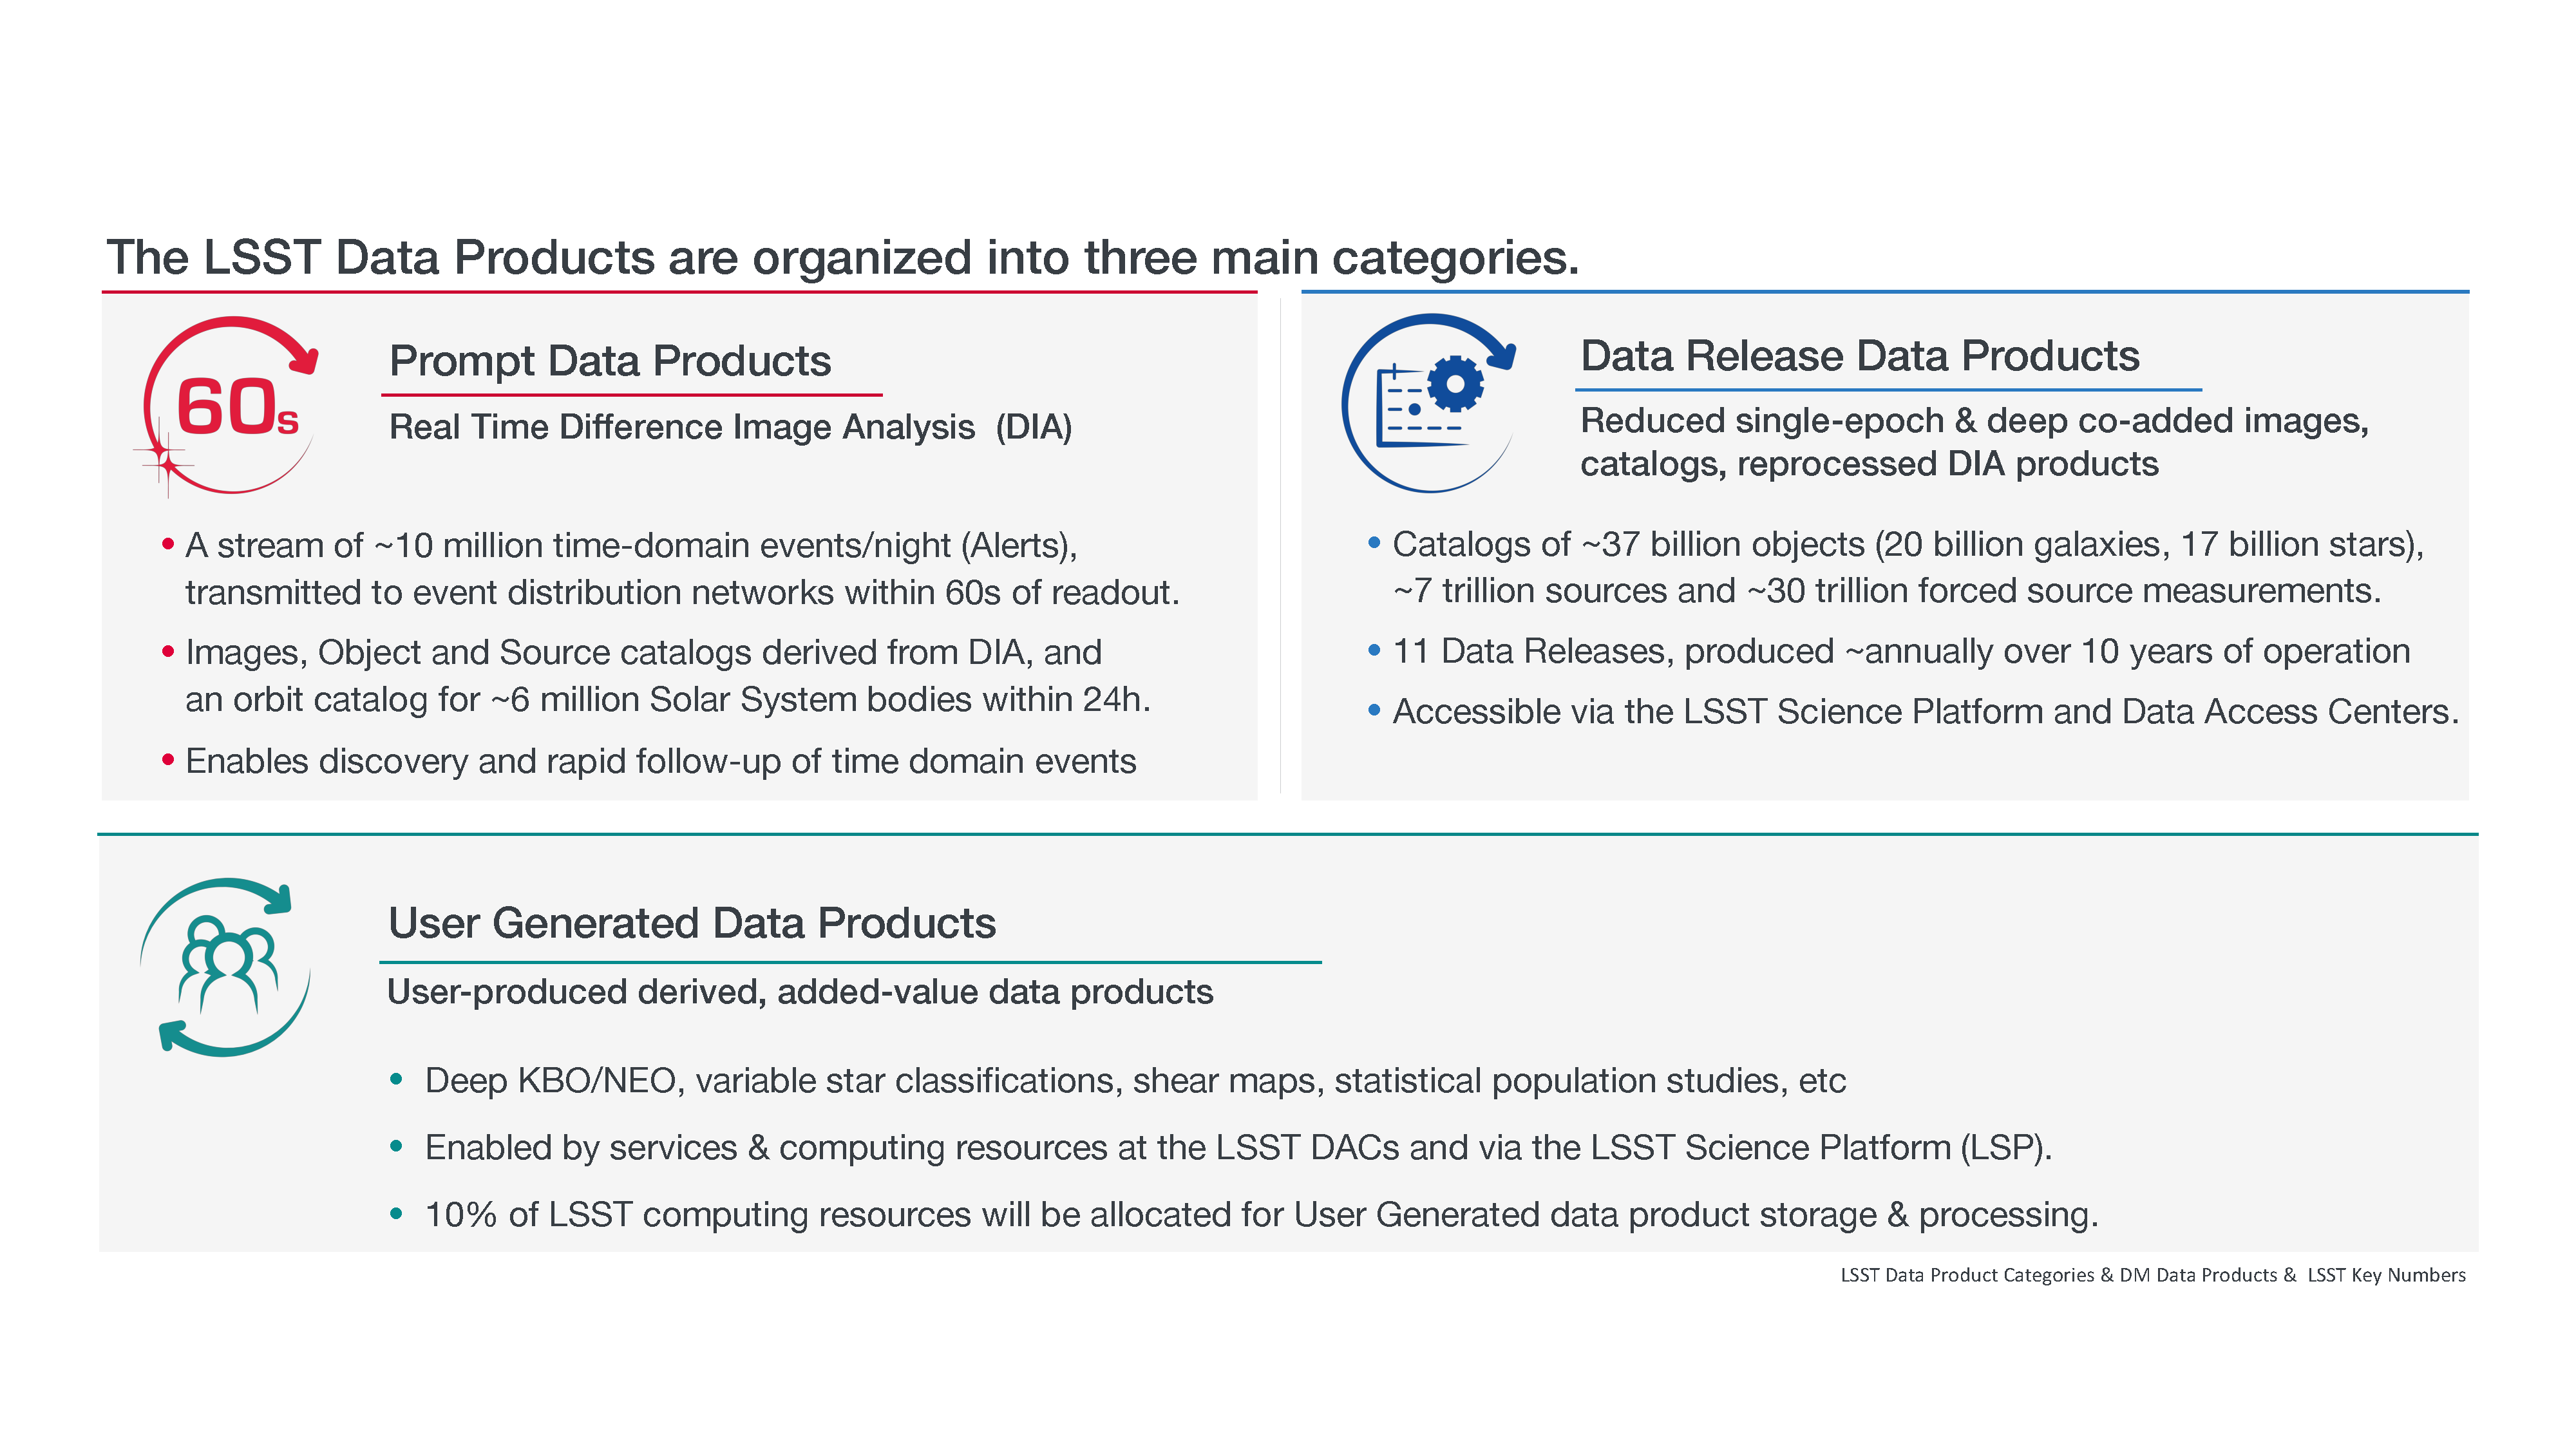
\includegraphics[width=1\textwidth]{DataProds}
{\tiny Leanne Guy}
}



\frame{\frametitle{Alerts: identify time varying object }
\begin{center}
\includegraphics[width=0.9\textwidth]{images/alertFlow}\\
\vspace{-5pt}
\hfill {\tiny \bf Figure from Eric Bellm}
\end{center}
}

\frame{\frametitle{Brokers  }
\begin{itemize}
\item LSST Mini Broker - Users can create filters that return
\begin{itemize}
\item a subset of LSST alerts based only on data in the alert packet
\item  can use lightcurve, variability parameters, colors, etc.,
\item no crossmatch to external catalogs
\item Runs in the LSST Data Access Center(-> users must have data rights)
\end{itemize}

 \item Community Alert Brokers -  further enabling science on alerts {\em e.g.}:
\begin{itemize}
\item Provide public access to alerts
\item Classification and Crossmatch to other catalogs or data streams
\item Provide filtering, visualization, and search
\item Coordinate scientific activity and/or followup observations
\item Aggregate alert annotations (community classifications, etc.)
\end{itemize}

\item {\color{red}Mini Broker capacity/Number of community brokers  limited by bandwidth}
\begin{itemize}
\item see \citeds{LDM-612}
\item Working out selection process for 2019
\end{itemize}

\end{itemize}
}



